\documentclass[11pt]{article}            % Report class in 11 points
\parindent0pt  \parskip10pt             % make block paragraphs
\usepackage{graphicx}
\usepackage{listings}
\graphicspath{ {images/} }
\usepackage{graphicx} %  graphics header file
\begin{document}
\begin{titlepage}
    \centering
  \vfill
    
\includegraphics[width=8cm]{uni_logo.png} \\ 
	\vskip2cm
    {\bfseries\Large
	Artificial Intelligence \\ (CS13217)\\
	
	\vskip2cm
	Lab Report 2
	 
	\vskip2cm
	}    

\begin{center}
\begin{tabular}{ l l  } 

Name: Kanza Afzal \\ 
Registration \#: & CSU-XS18-132 \\ 
Lab Report \#: & 02 \\ 
 Dated:&16-04-2018\\ 
Submitted To:& Mr. Usman Ahmed\\ 

 %\hline
\end{tabular}
\end{center}
    \v
    The University of Lahore, Islamabad Campus\\
Department of Computer Science \& Information Technology
\end{titlepage}


    
    {\bfseries\Large
\centering
	Experiment \# 2 \\

Implementing Tower of Hanoi Problem\\
	
	}    
 \vskip1cm
 \textbf {Objective}\\  To understand and implement the Tower of Hanoi Problem.
 
 \textbf {Software Tool} \\
1.  \\Dev

\section{Theory }              
The Tower of Hanoi is a mathematical game or puzzle. It consists of three rods, and a number of disks of different sizes which can slide onto any rod. The puzzle starts with the disks in a neat stack in ascending order of size on one rod, the smallest at the top, thus making a conical shape. \\
The objective of the puzzle is to move the entire stack to another rod, obeying the following simple rules:\\
1.	Only one disk can be moved at a time.\\
2.	Each move consists of taking the upper disk from one of the stacks and placing it on top of another stack i.e. a disk can only be moved if it is the uppermost disk on a stack.\\
3.	No disk may be placed on top of a smaller disk.\\ \\
With three disks, the puzzle can be solved in seven moves. 
The minimum number of moves required to solve a Tower of Hanoi puzzle is 2n - 1, where n is the number of disks.

\section{Task}  
\subsection{Procedure: Task 1 }     

\begin{figure*}
\centering
  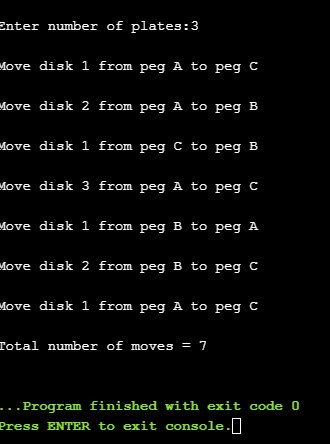
\includegraphics[width=24cm,height=12cm,keepaspectratio]{22.jpg}
\caption{Tower of Hanoi output}
\label{Figure:3}    
\end{figure*}
The minimum number of moves required to solve a Tower of Hanoi puzzle is 2n - 1, where n is the number of disks.

\subsection{Procedure: Task 2 }     

\begin{lstlisting}[language=C++]
int TOH(int,char,char,char);
 int main()
 {
   int n;
   printf("\nEnter number of plates:");
   scanf("%d",&n);
    int c = TOH(n,'A','C','B');
    printf("\n");
    printf("Total number of moves = %d \n ", c);
  return 0;
  }
int TOH(int n,char x,char y,char z)
{
   int count = 0;
   if(n>0){
       count = TOH(n-1, x, z, y);
       printf("\nMove disk %d from peg %c to peg %c\n", n, x, y);
       count++;
       count += TOH(n-1, z, y, x) ;
   }
   return count;
}
\end{lstlisting}

\section{Conclusion}  

 When the number of disks is 2 the number of moves it takes is 3, for 4 disks 15 and for 64 disks the program keeps running infinity loop
\end{document}                          % The required last line
